%----------------------------------------------------------------------------------------
% Preambulo y Configuración
%----------------------------------------------------------------------------------------

\documentclass[
    11pt,
    spanish,
    singlespacing,
    parskip,
    headsepline,
    bookmarks=true,
    unicode=true,
    pdftoolbar=true,
    pdfmenubar=true,
    pdffitwindow=false,
    colorlinks=true,
    linkcolor=blue,
    citecolor=blue,
    urlcolor=blue
]{MastersDoctoralThesis}

\usepackage[utf8]{inputenc} % Codificación de entrada UTF-8
\usepackage[T1]{fontenc}    % Codificación de salida para caracteres especiales
\usepackage{graphicx}       % Manejo de gráficos
\usepackage{eso-pic}        % Permite agregar fondos
\usepackage{hyperref}       % Manejo de hipervínculos y marcadores
\usepackage{biblatex}       % Manejo de bibliografía con Biber
\usepackage{url} % Para manejar URLs en referencias

\addbibresource{references.bib} % Enlace al archivo de referencias

% Redefinición de caracteres problemáticos en marcadores
\hypersetup{
    pdftitle={Título del Documento},
    pdfauthor={Autor del Documento},
    pdfkeywords={Sistemas Embebidos, Internet de las Cosas, Inteligencia Artificial},
    pdfstartview={FitH},
    unicode=true,
    colorlinks=true,
    linkcolor=blue,
    citecolor=blue,
    urlcolor=blue
}

\pdfstringdefDisableCommands{%
  \def\texttt#1{#1}%
  \def\textbf#1{#1}%
  \def\textit#1{#1}%
  \def\"{\"}%
  \def\~{~}%
  \def\'{'}%
  \def\^{}%
  \def\textunderscore{\_} % Manejo del subrayado en marcadores
}


% Definir comandos requeridos por la clase
\newcommand{\degreename}{Maestría en Ciencias} % Cambia según tu título
\newcommand{\univname}{Universidad Nacional de Ejemplo} % Cambia según tu universidad
\newcommand{\keywordnames}{Palabras clave:}
%----------------------------------------------------------------------------------------
% Documento Principal
%----------------------------------------------------------------------------------------

\begin{document}

% Configuración de la portada
\posgrado{Carrera / Maestría}
\keywords{Sistemas Embebidos, Internet de las Cosas, Inteligencia Artificial}

% Incluir la portada desde un archivo separado
%----------------------------------------------------------------------------------------
% PORTADA
%----------------------------------------------------------------------------------------
\begin{titlepage}
    % Fondo completo con el PDF que incluye la barra y el logo
    \AddToShipoutPictureBG*{\includegraphics[width=\paperwidth, height=\paperheight]{Figures/fondo.pdf}}

    % Contenido principal
    \begin{flushright}
        \setlength{\rightskip}{-2cm} % Ajusta la sangría derecha
        \vspace*{7.5cm} % Ajustar según la posición vertical deseada

        % Título
        {\fontfamily{phv}\bfseries\fontsize{33pt}{40pt}\selectfont
        Desarrollo de un sistema embebido para la gestión y monitoreo de cultivos verticales} \\[1.5cm]

        % Autor
        {\fontfamily{phv}\fontsize{20pt}{25pt}\selectfont
        Ing. José Luis Krüger} \\[1cm]

        % Carrera o Maestría (comentar o descomentar la línea correspondiente)
        {\fontfamily{phv}\fontsize{15pt}{20pt}\selectfont
        \textbf{Carrera de Especialización en Sistemas Embebidos}
        % \textbf{Carrera de Especialización en Internet de las Cosas} \\
        % \textbf{Carrera de Especialización en Inteligencia Artificial} \\
        % \textbf{Maestría en Sistemas Embebidos} \\
        % \textbf{Maestría en Internet de las Cosas} \\
        % \textbf{Maestría en Inteligencia Artificial Embebida} \\
        % \textbf{Maestría en Computación de Borde} \\
        % \textbf{Maestría en Inteligencia Artificial} \\
        } \\[2cm]

        % Director
        {\fontfamily{phv}\fontsize{11pt}{15pt}\selectfont
        \textbf{Director:} Esp. Ing. Mariano Campos (FIUBA)} \\[1cm]

        % Jurados
        {\fontfamily{phv}\fontsize{11pt}{15pt}\selectfont
        \textbf{Jurados:}} \\[0.5cm]
        {\fontfamily{phv}\fontsize{11pt}{15pt}\selectfont
        Jurado 1 (pertenencia)} \\ 
        {\fontfamily{phv}\fontsize{11pt}{15pt}\selectfont
        Jurado 2 (pertenencia)} \\ 
        {\fontfamily{phv}\fontsize{11pt}{15pt}\selectfont
        Jurado 3 (pertenencia)} \\[2cm]

        % Fecha y lugar
        {\fontfamily{phv}\itshape\fontsize{10pt}{12pt}\selectfont
        Ciudad de [lugar], [mes] de [año]} % Ejemplo: Ciudad de Córdoba, junio de 2025
    \end{flushright}
\end{titlepage}


% Configuración del contenido preliminar
\frontmatter % Usar numeración romana para las páginas preliminares
\pagestyle{plain} % Estilo de encabezado simple

%----------------------------------------------------------------------------------------
% Resumen
%----------------------------------------------------------------------------------------

\begin{abstract}
\addchaptertocentry{\abstractname} % Agregar resumen al índice
Este trabajo presenta el desarrollo, construcción, instalación y prueba de un dispositivo semiautomático de monitoreo y gestión para un cultivo hidropónico vertical. Su implementación requirió la aplicación de conocimientos en electrónica, programación, sistemas operativos de tiempo real, testing de software, diseño y ensamblaje de PCB, integración de sensores y protocolos de comunicación.

El sistema mejora la eficiencia del cultivo al minimizar los desperdicios y aumentar la productividad en comparación con los métodos tradicionales. Este avance representa un paso clave hacia la sostenibilidad y la optimización de la producción de alimentos en el futuro.
\end{abstract}

%----------------------------------------------------------------------------------------
% Agradecimientos
%----------------------------------------------------------------------------------------

\begin{acknowledgements}
\vspace{1.5cm}
Esta sección es para agradecimientos personales y es totalmente \textbf{OPCIONAL}.
\end{acknowledgements}

%----------------------------------------------------------------------------------------
% Índice
%----------------------------------------------------------------------------------------

\tableofcontents
\listoffigures
\listoftables

%----------------------------------------------------------------------------------------
% Dedicatoria
%----------------------------------------------------------------------------------------

\dedicatory{\textbf{Dedicado a... [OPCIONAL]}}

%----------------------------------------------------------------------------------------
% Capítulos
%----------------------------------------------------------------------------------------

\mainmatter % Iniciar numeración numérica para el contenido principal
\pagestyle{thesis} % Estilo de encabezado de tesis

% Incluir capítulos desde archivos separados
% Chapter 1

\chapter{Introducción general} % Main chapter title

\label{Chapter1} % For referencing the chapter elsewhere, use \ref{Chapter1} 
\label{IntroGeneral}

En este capítulo se expone la necesidad que dio origen al desarrollo del trabajo. Se presenta el concepto de cultivo vertical y el estado del arte de su integración con la tecnología. Asimismo, se explican el objetivo y los alcances del trabajo.

%----------------------------------------------------------------------------------------

% Define some commands to keep the formatting separated from the content 
\newcommand{\keyword}[1]{\textbf{#1}}
\newcommand{\tabhead}[1]{\textbf{#1}}
\newcommand{\code}[1]{\texttt{#1}}
\newcommand{\file}[1]{\texttt{\bfseries#1}}
\newcommand{\option}[1]{\texttt{\itshape#1}}
\newcommand{\grados}{$^{\circ}$}

%----------------------------------------------------------------------------------------

%\section{Introducción}

%----------------------------------------------------------------------------------------
\section{Agricultura vertical como solución sostenible}

%\LaTeX{} no es \textsc{WYSIWYG} (What You See is What You Get), a diferencia de los procesadores de texto como Microsoft Word o Pages de Apple o incluso LibreOffice en el mundo open-source. En lugar de ello, un documento escrito para \LaTeX{} es en realidad un archivo de texto simple o llano que \emph{no contiene formato} . Nosotros le decimos a \LaTeX{} cómo deseamos que se aplique el formato en el documento final escribiendo comandos simples entre el texto, por ejemplo, si quiero usar texto en itálicas para dar énfasis, escribo \verb|\it{texto}| y pongo el texto que quiero en itálicas entre medio de las llaves. Esto significa que \LaTeX{} es un lenguaje del tipo \enquote{mark-up}, muy parecido a HTML.

Con una población mundial que supera los 8000 millones de personas y continúa en crecimiento \cite{PEOPLE}, la agricultura enfrenta el desafío de volverse más eficiente y sostenible \cite{AGUA} \cite{FAO} \cite{SANTANDER}. En este contexto, los cultivos verticales emergen como una solución innovadora que optimiza el uso del espacio y los recursos, especialmente en entornos urbanos, donde el suelo es limitado y costoso.

Este tipo de agricultura utiliza técnicas como la hidroponía, que permite un uso preciso del agua, y la aeroponía, que maximiza el oxígeno disponible para las raíces. Además, las granjas verticales aprovechan áreas infrautilizadas, como edificios abandonados o naves industriales, y permiten cultivar alimentos en zonas donde la agricultura tradicional resulta dificil de desarrollar. Así, se logra una mayor densidad de cultivo y se contribuye a la sostenibilidad al reducir el uso de pesticidas y fertilizantes.

Aunque los cultivos verticales requieren un alto nivel de tecnología y tienen costes energéticos asociados, su capacidad para ahorrar recursos, disminuir la huella de carbono y fomentar la producción \cite{alhwarin2020vertical}.

Este método, también conocido como agricultura urbana, permite el crecimiento de plantas en interiores sin necesidad de luz solar directa, gracias a la aplicación de tecnologías agrícolas avanzadas. Estas optimizan las condiciones de cultivo, lo que facilita la propagación de plantas jóvenes y la producción de alimentos más saludables sin el uso de pesticidas.

Además, maximizan la producción al emplear sistemas de iluminación especializados de nueva generación, diseñados para estructuras multicapa. Gracias a esta tecnología, es posible obtener mayores rendimientos en un espacio reducido, consolidando a la agricultura vertical como una solución sostenible y eficiente para la producción de alimentos en entornos urbanos y con recursos limitados \cite{SANTANDER}.

\subsection{Tipos de cultivos verticales}

%https://agroquivir.com/agricultura-vertical-como-funciona-y-tipos/

%Si sos nuevo en \LaTeX{}, hay un muy buen libro electrónico - disponible gratuitamente en Internet como un archivo PDF - llamado, \enquote{A (not so short) Introduction to \LaTeX{}}. El título del libro es generalmente acortado a simplemente \emph{lshort}. Puede descargar la versión más reciente en inglés (ya que se actualiza de vez en cuando) desde aquí:
%\url{http://www.ctan.org/tex-archive/info/lshort/english/lshort.pdf}

%Se puede encontrar la versión en español en la lista en esta página: \url{http://www.ctan.org/tex-archive/info/lshort/}

Existen distintos tipos de agricultura vertical, que optimizan el crecimiento de las plantas sin grandes extensiones de suelo y emplean estructuras especializadas para maximizar la producción.
A continuación se describen los principales tipos de cultivos verticales y sus características:

\subsubsection{Hidroponía}
La hidroponía es un método de cultivo sin suelo que suministra nutrientes a las plantas a través de una solución acuosa, con raíces en un medio inerte como lana de roca o perlita. Es un sistema eficiente en el uso de agua, permite un control preciso de nutrientes y favorece una mayor densidad de cultivo y un crecimiento más rápido que los métodos tradicionales \cite{SANTANDER} \cite{CULTIVOS:TIPOS}.
\subsubsection{Aeroponía}
La aeroponía es un método de cultivo en el que las raíces de las plantas quedan suspendidas en el aire y se rocían con una solución nutritiva. Maximiza la oxigenación, acelera el crecimiento y optimiza el uso de nutrientes, aunque requiere un control preciso para evitar la desecación de las raíces \cite{SANTANDER} \cite{CULTIVOS:TIPOS}.
\subsubsection{Acuaponía}
La acuaponía combina la cría de peces con la hidroponía, utilizando los desechos de los peces como fertilizante para las plantas, mientras estas purifican el agua. Es un sistema sostenible y eficiente que minimiza el desperdicio, promueve la biodiversidad y es viable en entornos urbanos y rurales \cite{CULTIVOS:TIPOS}.

%Acá tiene un ejemplo de una ``subsubsección'' que es el cuarto nivel de ordenamiento del texto, después de capítulo, sección y subsección.  Como se puede ver, las subsubsecciones no van numeradas en el cuerpo del documento ni en el índice.  El formato está definido por la plantilla y no debe ser modificado.

\subsection{Sistemas de agricultura vertical más conocidos}
Los sistemas de agricultura vertical varían según el tipo de cultivo y la técnica más adecuada para cada necesidad.
A continuación se describen los principales sistemas de cultivos verticales y sus características:

\subsubsection{Sistemas de torre}
Las torres verticales permiten el cultivo de plantas en estructuras cilíndricas apiladas, con el fin de maximizar el uso del espacio y facilitar tanto la recolección como el mantenimiento. Este sistema es ideal para cultivos de hoja verde y hierbas, y se integra fácilmente en espacios urbanos como balcones y terrazas \cite{CULTIVOS:TIPOS}.

\subsubsection{Sistemas en rack o estanterías}
Estos sistemas emplean estanterías apiladas donde las plantas crecen en bandejas o contenedores, son ideales para invernaderos y ambientes controlados. Facilitan el riego, la recolección y el monitoreo, al mismo tiempo que se optimiza el uso del espacio.
Los sistemas en rack o estanterías son especialmente útiles para cultivos que requieren diferentes niveles de luz y humedad \cite{CULTIVOS:TIPOS}.

\subsubsection{Sistemas montados en pared}
En estos sistemas, las plantas crecen en módulos montados en paredes. Su integración en la arquitectura no solo optimiza el espacio, sino que también aporta beneficios estéticos y funcionales.
Los jardines verticales pueden mejorar la calidad del aire y contribuir al aislamiento térmico de los edificios \cite{CULTIVOS:TIPOS}.

\subsubsection{Sistemas de bastidor en A}
El bastidor en forma de ``A`` proporciona una estructura estable y accesible para el cultivo vertical, lo que a su vez facilita el acceso a la luz y el riego.
Este diseño es particularmente útil para cultivos que necesitan un soporte adicional, como tomates y pepinos, y puede ser utilizado tanto en interiores como en exteriores \cite{CULTIVOS:TIPOS}.

\subsubsection{Sistemas de contenedores}
Estos sistemas utilizan contenedores apilables que pueden moverse y configurarse según las necesidades, adaptándose a diversos entornos y tipos de cultivo.
Los contenedores son ideales para cultivos modulares y pueden ser personalizados para optimizar el uso del espacio y los recursos \cite{CULTIVOS:TIPOS}.
%Si estás escribiendo un documento con mucho contenido matemático, entonces es posible que desees leer el documento de la AMS (American Mathematical Society) llamado, \enquote{A Short Math Guide for \LaTeX{}}. Se puede encontrar en línea en el siguiente link: \url{http://www.ams.org/tex/amslatex.html} en la sección \enquote{Additional Documentation} hacia la parte inferior de la página.


%----------------------------------------------------------------------------------------

\section{Motivación}

Este trabajo surge como un desarrollo de interés personal, impulsado por el deseo de contribuir positivamente al desarrollo sustentable y la optimización de los recursos naturales en la producción de alimentos. En la actualidad, el crecimiento de la población mundial y el aumento en la demanda de productos agrícolas presentan grandes desafíos ambientales y económicos.

La producción tradicional de alimentos enfrenta dificultades debido a la explotación intensiva de suelos, el uso excesivo de fertilizantes y pesticidas y el desperdicio de recursos esenciales como el agua. Con el fin de maximizar sus ganancias, muchas empresas recurren a métodos poco sostenibles que generan un impacto ambiental negativo, y afectan la biodiversidad, la calidad del suelo y el bienestar de las comunidades locales que dependen de estas fuentes de producción.

Uno de los problemas más críticos en la agricultura tradicional es el significativo desperdicio de agua en el riego. Se estima que se desperdicia hasta el 84 \% del agua utilizada para riego \cite{CLARIN}. Esta pérdida ocurre principalmente por evaporación, drenaje o absorción ineficiente. En un contexto donde la crisis hídrica es una amenaza global, desarrollar sistemas más sostenibles se vuelve una necesidad urgente.

Por otro lado, existe una creciente preocupación entre los consumidores sobre la calidad y procedencia de los alimentos. Cada vez más personas optan por un estilo de vida saludable, adoptando hábitos de consumo responsables, como el vegetarianismo, el veganismo y el autocultivo. Sin embargo, muchos de estos consumidores no cuentan con espacios adecuados ni conocimientos técnicos para producir sus propios alimentos, lo que genera una gran oportunidad para soluciones tecnológicas que faciliten la agricultura doméstica.

A partir de estas problemáticas, nació la motivación para desarrollar un sistema hidropónico inteligente, que no solo optimice el uso del agua, sino que también permita una gestión eficiente del cultivo con mínima intervención del usuario. Este trabajo ofrece una alternativa viable y escalable para la producción de alimentos frescos, reduce la dependencia de sistemas agrícolas tradicionales y promueve un modelo más sustentable para el futuro.


\section{Estado del arte}
Durante la etapa de investigación, se llevó a cabo una búsqueda de productos comerciales tanto en el mercado local como en el internacional. Se identificaron diversas soluciones con características similares al sistema desarrollado.

A continuación, se describen los productos identificados.

\subsubsection{NIDO PRO}
El NIDO PRO, figura \ref{fig:nido_pro}, es un sistema hidropónico inteligente para cultivos verticales que permite controlar la solución nutritiva a través de una aplicación móvil. Facilita la gestión del pH y la conductividad eléctrica (CE), con algoritmos que realizan comprobaciones diarias para garantizar la estabilidad de la solución nutritiva. Además, admite hasta cuatro ranuras para fertilizantes líquidos y ajustes de pH, lo que optimiza el proceso de nutrición de las plantas \cite{NIDO:PRO}.

\begin{figure}[h]
	\centering
	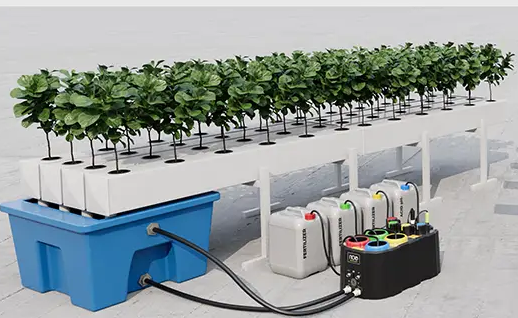
\includegraphics[height=8cm]{./Figures/nido:pro.png}
	\caption{Ilustración del módulo NIDO PRO conectado a un sistema hidropónico horizontal.}
	\label{fig:nido_pro}
\end{figure}

%https://www.agrointec.com/producto/nidopro-sistema-hidroponico-inteligente-cultivo-vertical/?utm_source=chatgpt.com

\subsubsection{Xiaomi Mi Flower Care Plant Sensor}
El Xiaomi Mi Flower Care Plant Sensor, figura \ref{fig:xiaomi}, monitorea variables ambientales como luz, humedad, nutrientes y temperatura del sustrato. Los sensores se conectan a aplicaciones móviles, lo que permite realizar un seguimiento detallado y controlar las condiciones del cultivo de manera precisa \cite{XIAOMI}.

\begin{figure}[h]
	\centering
	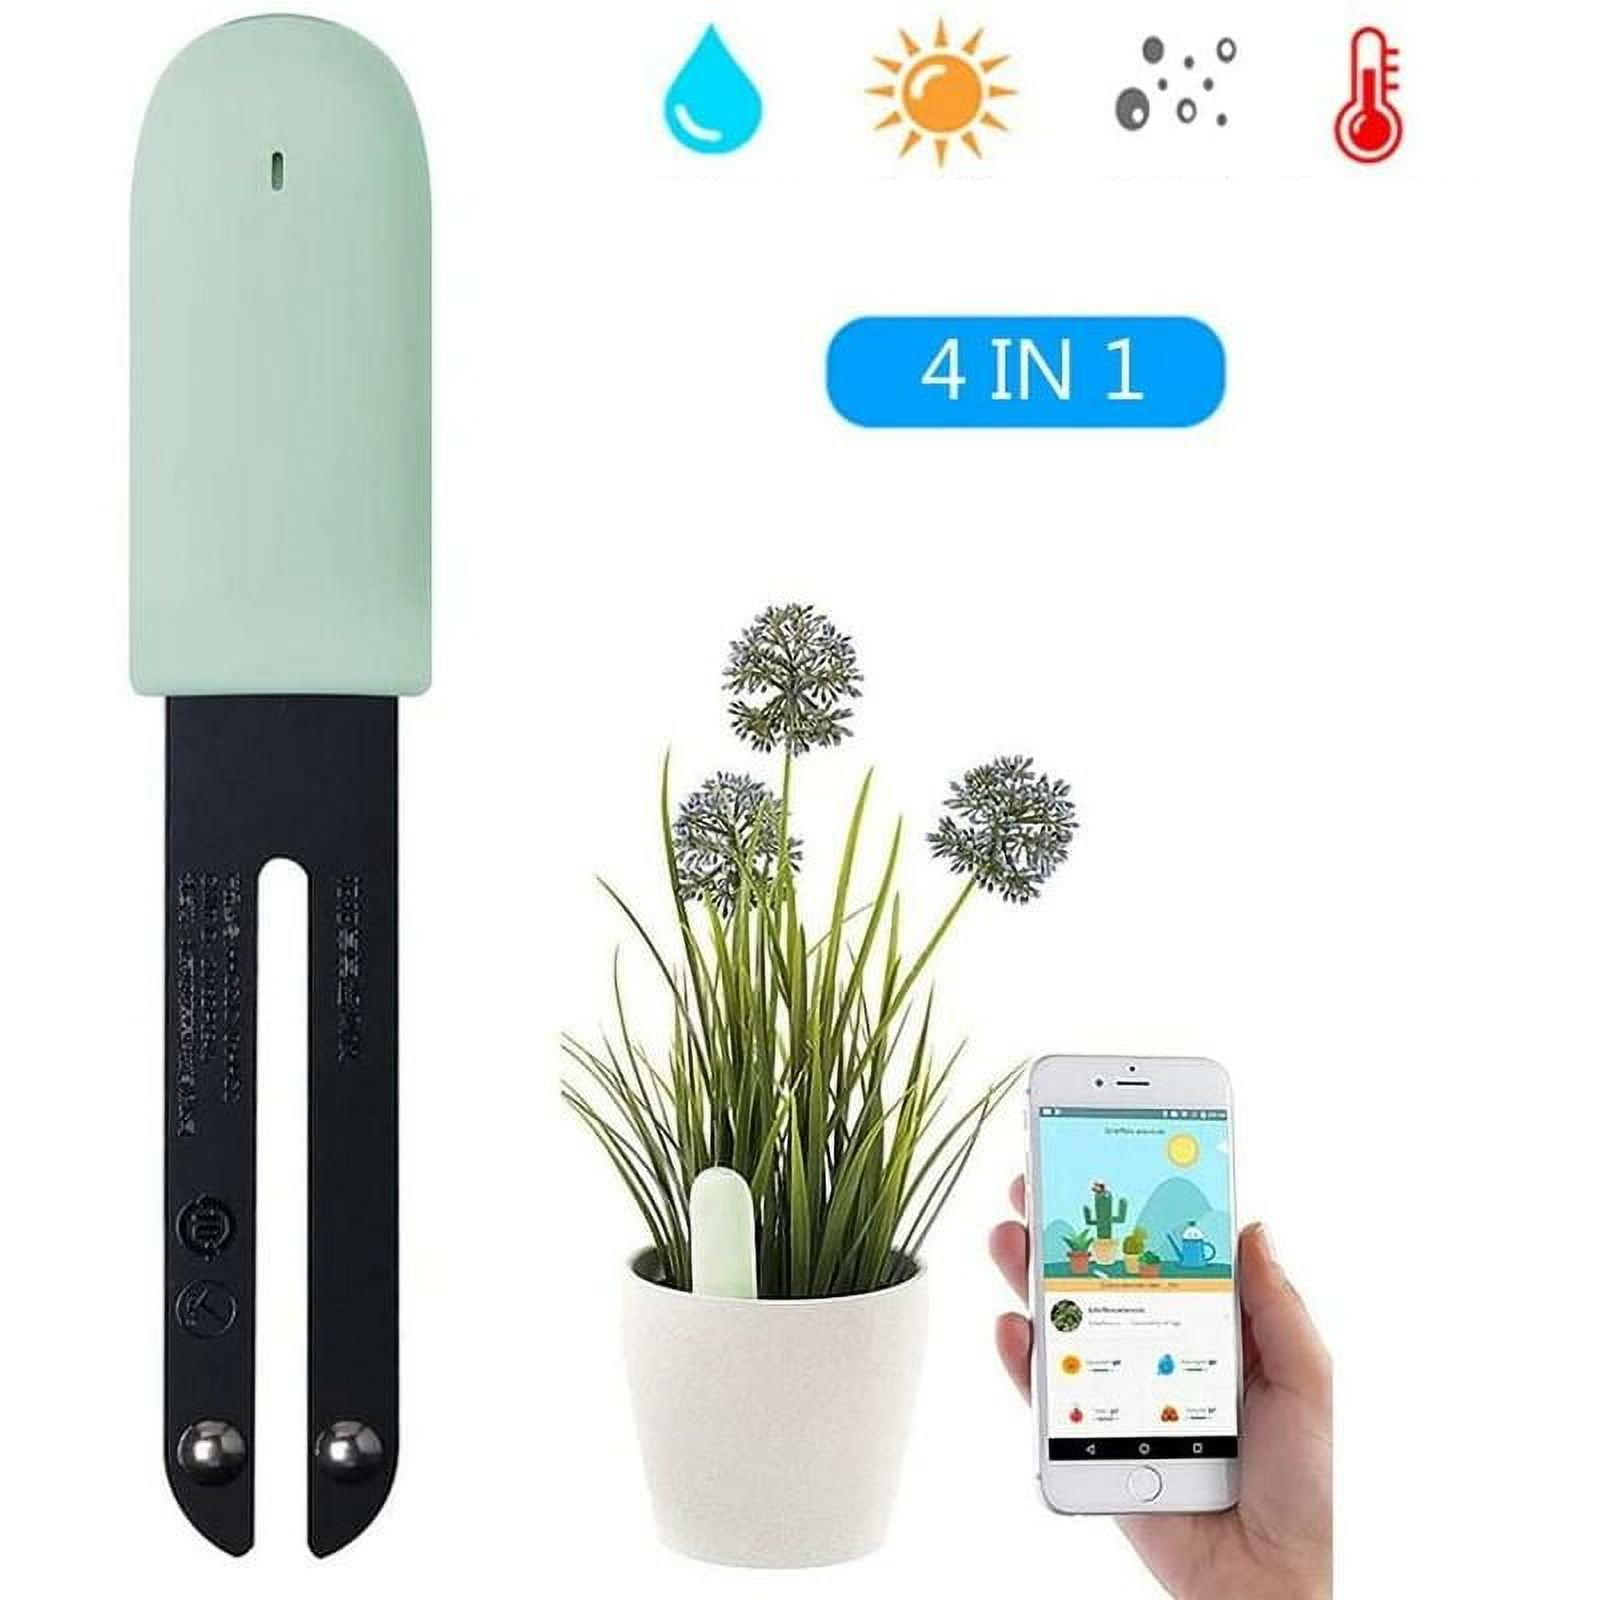
\includegraphics[height=8cm]{./Figures/xiaomi.jpg}
	\caption{Ilustración del dispositivo Xiaomi Mi Flower Care Plant Sensor y sus prestaciones.}
	\label{fig:xiaomi}
\end{figure}

%https://elpais.com/tecnologia/tu-tecnologia/2024-12-07/dispositivos-tecnologicos-para-que-tus-plantas-sean-la-envidia-de-cualquiera.html?utm_source=chatgpt.com

\subsubsection{Kit de Riego Hydro de Konyks}
El sistema de riego inteligente Konyks, figura \ref{fig:kit_konyks}, permite controlar la llave de paso de forma remota mediante una aplicación móvil y asistentes de voz como Alexa, Google Home o Siri. Incorpora un medidor de caudal para monitorear el consumo de agua y una toma con relé RF que amplía la conectividad hasta 60 m y permite gestionar hasta cuatro grifos. Además, ofrece automatización programable según el clima y los horarios, lo que optimiza el uso del agua y facilita la gestión del riego desde cualquier lugar \cite{KONIX}.

\begin{figure}[h]
	\centering
	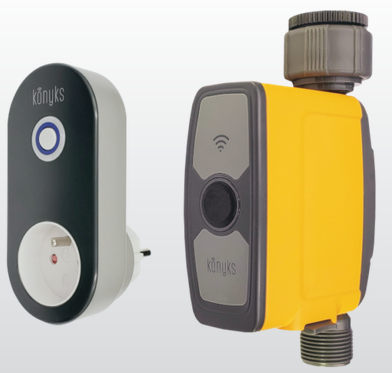
\includegraphics[height=8cm]{./Figures/kit_konyks.png}
	\caption{Sistema de riego conectado Konyks.}
	\label{fig:kit_konyks}
\end{figure}

%https://elpais.com/tecnologia/tu-tecnologia/2024-12-07/dispositivos-tecnologicos-para-que-tus-plantas-sean-la-envidia-de-cualquiera.html?utm_source=chatgpt.com

\subsubsection{Smart 9 Pro de Click \& Grow}
El Smart Garden 9 PRO, figura \ref{fig:smart_garden}, es un sistema de cultivo doméstico automatizado con control a través de una aplicación. Ofrece riego automático, iluminación ajustable tanto por control táctil como desde la app, y un suministro equilibrado de nutrientes y oxígeno en las raíces. Permite cultivar hierbas, frutas, ensaladas y flores durante todo el año, con la opción de utilizar cápsulas presembradas (más de 50 variedades disponibles) o semillas propias. Incluye un set inicial con cápsulas de tomate, albahaca y lechuga \cite{SMART:9}.

\begin{figure}[h]
	\centering
	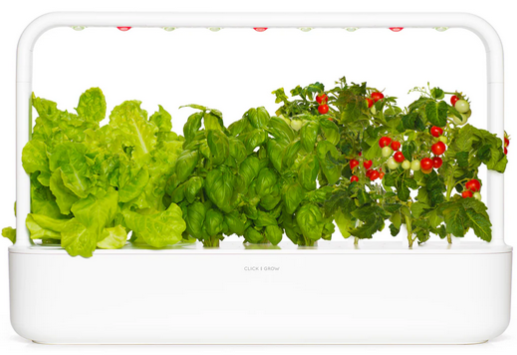
\includegraphics[height=8cm]{./Figures/smart_garden.png}
	\caption{Módulo Smart Garden 9 PRO.}
	\label{fig:smart_garden}
\end{figure}

%https://elpais.com/tecnologia/tu-tecnologia/2024-12-07/dispositivos-tecnologicos-para-que-tus-plantas-sean-la-envidia-de-cualquiera.html?utm_source=chatgpt.com

\section{Objetivos y alcances}

A continuación se presentan los objetivos del trabajo:

\subsection{Objetivos}
\begin{itemize}
    \item Desarrollar un prototipo de sistema hidropónico automatizado para monitoreo y gestión eficiente del cultivo.
    \item Implementar la conexión de sensores para medir temperatura, humedad, pH, conductividad eléctrica, nivel de agua e intensidad lumínica.
    \item Diseñar una interfaz web y móvil que permita la supervisión y configuración remota del sistema.
    \item Evaluar el rendimiento del sistema en comparación con métodos tradicionales, midiendo eficiencia y productividad.
    \item Poner en práctica los conocimientos adquiridos a lo largo de la carrera de especialización en sistemas embebidos.
\end{itemize}

\subsection{Alcances}

A continuación de presentan los alcances del trabajo:

\begin{itemize}
    \item El sistema permite el monitoreo en tiempo real y la gestión automatizada del riego, iluminación y ventilación.
    \item El dispositivo se enfocó en cultivos hidropónicos verticales de pequeña y mediana escala.
    \item Se realizaron pruebas de funcionamiento y validación en un entorno controlado, pero no se contempló una implementación comercial en esta etapa.
\end{itemize}

%Si estás familiarizado con \LaTeX{}, entonces podés explorar la estructura de directorios de esta plantilla y proceder a personalizarla agregando tu información en el bloque \emph{INFORMACIÓN DE LA PORTADA} en el archivo \file{memoria.tex}.  

%Se puede continuar luego modificando el resto de los archivos siguiendo los lineamientos que se describen en la sección \ref{sec:FillingFile} en la página \pageref{sec:FillingFile}.

%Debés asegurarte de leer el capítulo \ref{Chapter2} acerca de las convenciones utilizadas para las Memoria de los Trabajos Finales de la \degreename.

%Si sos nuevo en \LaTeX{}, se recomienda que continúes leyendo el documento ya que contiene información básica para aprovechar el potencial de esta herramienta.


%----------------------------------------------------------------------------------------
\chapter{Introducción específica} % Main chapter title

\label{Chapter2}

%----------------------------------------------------------------------------------------
%	SECTION 1
%----------------------------------------------------------------------------------------
%Todos los capítulos deben comenzar con un breve párrafo introductorio que indique cuál es el contenido que se encontrará al leerlo.  La redacción sobre el contenido de la memoria debe hacerse en presente y todo lo referido al proyecto en pasado, siempre de modo impersonal.
En el presente capítulo se describen los componentes de hardware, software, protocolos de comunicación y plataformas utilizados para realizar el trabajo.

\section{Componentes principales del hardware}
\label{sec:hw:components}

En esta sección se describen los módulos de hardware de terceros utilizados en el trabajo.

\subsection{ESP32-DevKitC}
%https://docs.espressif.com/projects/esp-dev-kits/en/latest/esp32/esp32-devkitc/index.html

La placa ESP32-DevKitC V4, figura \ref{fig:devkit}, es una placa de desarrollo basada en el SoC (\textit{System On Chip}) ESP32 de Espressif Systems. Es una placa popular y versátil ampliamente utilizada por desarrolladores, ingenieros y aficionados para la creación de prototipos y el desarrollo de proyectos de internet de las cosas o IoT (del inglés \textit{Internet of Things}), sistemas embebidos y otras aplicaciones \cite{DEV:KIT}.

Cacterísticas generales:

\begin{itemize}
	\item Basada en diferentes módulos ESP32.
	\item Microcontrolador con arquitectura de uno o dos núcleos de 32 bits (típicamente Tensilica LX6) con velocidades de reloj de hasta 240 MHz.
	\item Memoria SRAM integrada (con opciones de PSRAM externa en algunos módulos como los WROVER).
	\item Memoria flash integrada para almacenamiento de firmware.
	\item Conectividad Wi-Fi 802.11 b/g/n (2.4 GHz) integrada.
	\item Conectividad bluetooth (classic y low energy) integrada.
	\item La mayoría de los pines I/O del módulo ESP32 están disponibles a través de pines header para una fácil conexión.
	\item Permite la conexión de periféricos con cables jumper o el montaje en una placa de pruebas.
	\item Conector micro USB para alimentación y comunicación.
	\item Botones de reset y boot integrados para facilitar la programación.
	\item Compatible con múltiples entornos de desarrollo (ESP-IDF, Arduino IDE, MicroPython).
\end{itemize}

\begin{figure}[h]
\centering
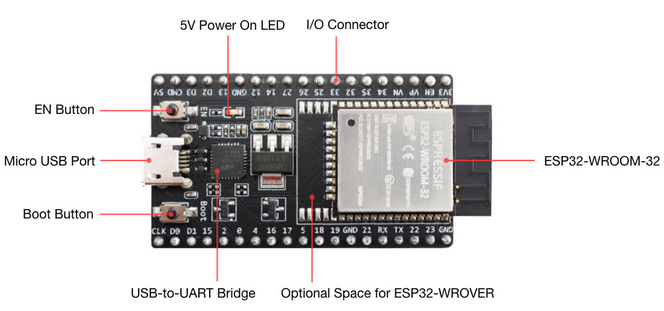
\includegraphics[scale=.5]{./Figures/devkit.png}
	\caption{ESP32-DevKitC V4 con el módulo ESP32-WROOM-32 integrado\protect\footnotemark.}
	\label{fig:devkit}
\end{figure}

\footnotetext{Imagen tomada de \url{https://docs.espressif.com/projects/esp-dev-kits/en/latest/esp32/esp32-devkitc/user_guide.html\#overview}}



\subsection{Módulo sensor PH-4502C}
El sensor de pH analógico PH-4502C, figura \ref{fig:ph}, es un módulo electrónico diseñado para medir el grado de acidez de soluciones líquidas, típicamente el modelo E201-BNC \cite{PH:4502C}. Este sensor proporciona una salida de tensión analógica que es proporcional al nivel de pH detectado por el electrodo.

Características:

\begin{itemize}
	\item Módulo electrónico compatible con electrodos de pH con conector BNC.
	\item Rango de detección de pH de 0 a 14.
	\item Salida analógica que varía, entre 0 y 5 VDC, con el pH del liquido.
	\item Requiere una alimentación de voltaje de 5V DC.
	\item Corriente de operación entre 5 y 10 mA.
	\item Temperatura de operación del módulo generalmente entre -10 °C y 50 °C.
	\item Incorpora un potenciómetro para el ajuste del offset o calibración.
	\item El electrodo tiene un tiempo de estabilización de respuesta de aproximadamente 1 minuto.
\end{itemize}

\begin{figure}[h]
\centering
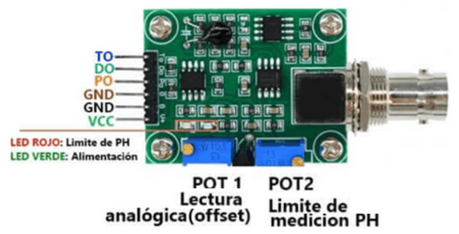
\includegraphics[scale=.5]{./Figures/ph.png}
	\caption{Distribución de pines del módulo PH-4502C\protect\footnotemark.}
	\label{fig:ph}
\end{figure}

\footnotetext{Imagen tomada de \url{https://uelectronics.com/producto/sensor-de-ph-liquido/?srsltid=AfmBOop9186NUUqLe2lmdM_tZTSfz79gsdcGSMFpg6aQvBxj-Fu9oF5t}}



%https://uelectronics.com/producto/sensor-de-ph-liquido/?srsltid=AfmBOop9186NUUqLe2lmdM_tZTSfz79gsdcGSMFpg6aQvBxj-Fu9oF5t

\subsection{Módulo medidos de solidos disueltos totales}

El medidor de sólidos disueltos totales o TDS (del inglés \textit{Total Dissolved Solids}) Meter 1.0, figura \ref{fig:tds}, es un sensor o módulo electrónico diseñado para medir la cantidad total de sustancias orgánicas e inorgánicas disueltas en un líquido, expresada típicamente en partes por millón (ppm) o miligramos por litro (mg/l) \cite{TDS}. Este tipo de sensor se utiliza para evaluar la calidad del agua en diversas aplicaciones como hidroponía, acuicultura, tratamiento de aguas y monitoreo ambiental.

Características:

\begin{itemize}
	\item Requiere alimentación de 3.3 a 5.5 VDC.
	\item Salida analógica de 0 a 2.3 VDC (proporcional a TDS).
	\item Rango de medición típico de 0 a 1000 ppm.
	\item Incluye sonda impermeable con electrodos.
	\item Interfaz de 3 pines (VCC, GND, output).
	\item Conector para la sonda (2 pines).
	\item Compensación de temperatura.
\end{itemize}


\begin{figure}[h]
\centering
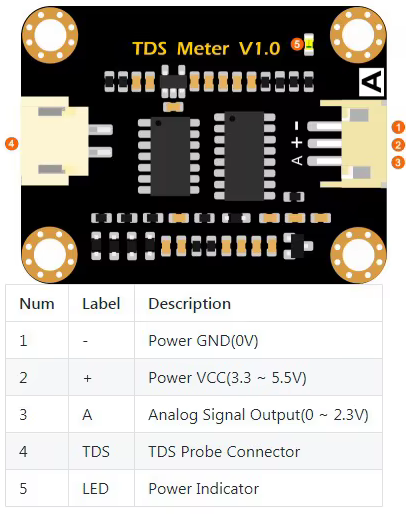
\includegraphics[scale=.5]{./Figures/tds.png}
	\caption{Ilustración del módulo sensor TDS meter v1.0\protect\footnotemark.}
	\label{fig:tds}
\end{figure}

\footnotetext{Imagen tomada de \url{https://www.digikey.be/htmldatasheets/production/2799469/0/0/1/sen0244.html}}



\subsection{Sensor de humedad capacitivo V2.0}

El sensor de humedad capacitivo V2.0, figura \ref{fig:moisture}, mide los niveles de humedad del medio mediante detección capacitiva en lugar de resistiva, como otros sensores disponibles. Fabricado con material resistente a la corrosión, ofrece una vida útil prolongada al insertarse en el sustrato alrededor de las plantas \cite{MOISTURE}.

\begin{itemize}
	\item Requiere alimentación de 3.3 a 5.5 VDC.
	\item Corriente de operación de 5 mA.
	\item Salida analógica.
	\item Incluye un regulador de tensión integrado compatible con MCUs de 3.3V y 5V.
\end{itemize}


\begin{figure}[h]
\centering
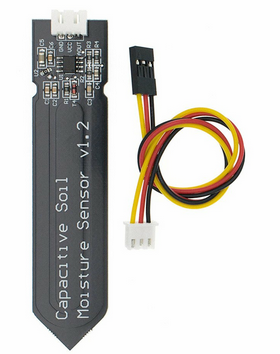
\includegraphics[scale=.5]{./Figures/moisture.png}
	\caption{Módulo sensor de humedad capacitivo\protect\footnotemark.}
	\label{fig:moisture}
\end{figure}

\footnotetext{Imagen tomada de \url{https://probots.co.in/soil-moisture-sensor-capacitive-v1-2.html}}


\subsection{Sensor de temperatura digital DS18B20}

El DS18B20, figura \ref{fig:ds18b20}, es un sensor de temperatura digital que proporciona mediciones en grados celsius con una resolución configurable de 9 a 12 bits \cite{DS18B20}. Este sensor se comunica a través de un bus 1-Wire, lo que significa que solo requiere una línea de datos (además de tierra) para la comunicación con un micontrolador. Cada DS18B20 tiene un código de serie único de 64 bits grabado en fábrica, lo que permite que múltiples sensores funcionen en el mismo bus 1-Wire, lo que permite la creación de redes de sensores de temperatura distribuidos.

Características:

\begin{itemize}
	\item Requiere alimentación de 3.3 a 5.5 VDC.
	\item Rango de medición de temperatura: -55 °C a +125 °C (-67 °F a +257 °F).
	\item Precisión: ±0.5 °C en el rango de -10 °C a +85 °C.
	\item Resolución configurable: 9, 10, 11 o 12 bits (por defecto 12 bits).
	\item Interfaz de comunicación: 1-Wire (requiere un solo pin digital).
	\item Cada sensor tiene una dirección única de 64 bits.
	\item Puede alimentarse a través de la línea de datos (\textit{parasite power}) o con una fuente externa.
	\item Tiempo de conversión de temperatura: hasta 750 ms (para resolución de 12 bits).
	\item Disponible en encapsulado TO-92 y en versiones con sonda impermeable.
\end{itemize}


\begin{figure}[h]
\centering
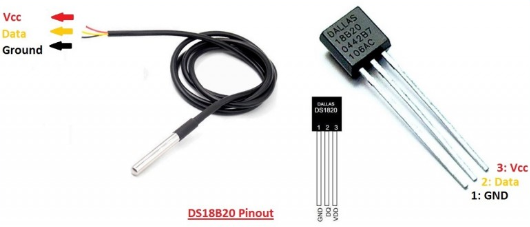
\includegraphics[scale=.5]{./Figures/ds18b20.png}
	\caption{Pinout del sensor DS18B20 y presentación del chip con su vaina protectora característica\protect\footnotemark.}
	\label{fig:ds18b20}
\end{figure}

\footnotetext{Imagen tomada de \url{https://tienda.ityt.com.ar/sensor-temp-hum-ic/1694-sensor-temperatura-ds18b20-18b20-1-wire-one-wire-itytarg.html}}


%https://tienda.ityt.com.ar/sensor-temp-hum-ic/1694-sensor-temperatura-ds18b20-18b20-1-wire-one-wire-itytarg.html

\subsection{Sensor de luz ambiental digital BH1750}

El circuito integrado BH1750, figura \ref{fig:BH1750}, es un sensor de luz ambiental digital con interfaz de bus I2C (\textit{Inter-Integrated Circuit}) \cite{BH1750}. Este sensor es capaz de detectar un amplio rango de intensidad luminosa con alta resolución, desde 1 hasta 65535 lux. El chip proporciona una salida digital directa, eliminando la necesidad de cálculos complejos.

Características:

\begin{itemize}
	\item Requiere alimentación de 3.3 a 5.5 VDC.
	\item Interfaz de comunicación I2C.
	\item Rango de medición de 1 a 65535 lux.
	\item Resolución: 16 bits.
\end{itemize}

\begin{figure}[h]
\centering
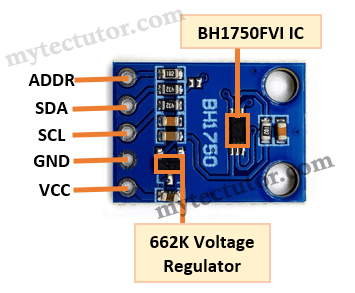
\includegraphics[scale=.5]{./Figures/BH1750.png}
	\caption{Pinout del módulo de adaptación del sensor BH1750\protect\footnotemark.}
	\label{fig:BH1750}
\end{figure}

\footnotetext{Imagen tomada de \url{https://mytectutor.com/bh1750-ambient-light-sensor-with-arduino/}}


%https://mytectutor.com/bh1750-ambient-light-sensor-with-arduino/


\section{Componentes principales del software}
\label{sec:sw:components}
En esta sección se describen las herramientas de software de terceros utilizados en el trabajo.


\subsection{ESP-IDF}

ESP-IDF (\textit{Espressif IoT Development Framework}) es un conjunto de herramientas de desarrollo integral provisto por Espressif Systems. Este framework facilita la creación de firmware para su línea de SoCs ESP32 y ESP8266. Incluye un sistema operativo en tiempo real (FreeRTOS), bibliotecas con APIs para diversos periféricos y protocolos (Wi-Fi, bluetooth, TCP/IP), compilador (basado en GCC), depurador (GDB) y utilidades para la construcción, flasheo y monitoreo de proyectos. ESP-IDF permite a los desarrolladores escribir aplicaciones en C o C++, quienes aprovechan así la potencia y la conectividad de los chips de Espressif \cite{ESPIDF}.


\subsection{FreeRTOS}

FreeRTOS es un sistema operativo en tiempo real (RTOS) popular y de código abierto. Ofrece un núcleo pequeño y eficiente, apropiado para microcontroladores y sistemas con recursos limitados. Proporciona mecanismos de multitarea, como hilos (tareas), gestión de memoria, sincronización y comunicación entre tareas (semáforos, mutexes, colas). Facilita la organización y la gestión de la ejecución de múltiples funciones de manera concurrente y determinista, crucial para aplicaciones de tiempo real. Su portabilidad permite su uso en una amplia variedad de arquitecturas de procesadores \cite{FREERTOS}.

\subsection{Ceedling}

Ceedling es un framework de construcción y prueba para proyectos de software embebido en C. Automatiza tareas como la compilación, el enlazado y la ejecución de pruebas unitarias. Integra herramientas como Unity (para escribir pruebas), CMock (para crear objetos simulados) y Ruby (como lenguaje de automatización). Facilita la adopción de prácticas de desarrollo basadas en pruebas (TDD) y asegura la calidad del código mediante la verificación automatizada de unidades de software individuales. Proporciona una estructura organizada para la gestión de pruebas y la generación de informes \cite{CEEDLING}.

\subsection{React Native}
React Native es un framework de código abierto desarrollado por Meta. Permite la creación de aplicaciones móviles para plataformas iOS y Android desde una única base de código JavaScript. Utiliza los mismos bloques de construcción de la interfaz de usuario que las aplicaciones nativas. Esto resulta en aplicaciones con apariencia y rendimiento nativos. Una gran comunidad y un amplio ecosistema de bibliotecas lo respaldan \cite{reactnative}.

\section{Protocolos de comunicación empleados}

A continuación de detallan los protocolos de comunicación empleados en la realización del trabajo.

\subsection{HTTP}
HTTP (\textit{Hypertext Transfer Protocol}) es un protocolo de aplicación fundamental para la red de internet mundial. Define cómo los clientes (navegadores web) solicitan recursos (páginas web, imágenes, etc.) a los servidores y cómo estos responden. Utiliza un modelo de petición-respuesta. Las peticiones HTTP incluyen un método (GET, POST, PUT, DELETE, etc.) que indica la acción que el cliente desea realizar. Las respuestas HTTP contienen un código de estado que informa sobre el resultado de la petición. HTTP es un protocolo sin estado, lo que significa que cada petición es independiente de las anteriores \cite{HTTP}.

\subsection{I2C}
I2C (Inter-Integrated Circuit) es un protocolo de comunicación serial síncrono, multi-maestro/esclavo, de baja velocidad y corta distancia. Utiliza solo dos líneas bidireccionales: SDA (datos seriales) y SCL (reloj serial), ambas conectadas a través de resistencias pull-up. Permite que múltiples dispositivos (maestros y esclavos) se comuniquen entre sí en el mismo bus. Cada dispositivo es direccionable por un identificador único de 7 o 10 bits. Los maestros inician la comunicación y controlan el reloj, mientras que los esclavos responden a las peticiones de los maestros. Es ampliamente utilizado para conectar microcontroladores con periféricos de baja velocidad como sensores, EEPROMs y pantallas \cite{I2C}.

\subsection{1-Wire}
1-Wire es un protocolo de comunicación serial semidúplex diseñado por Dallas Semiconductor (ahora Analog Devices). Utiliza un único conductor para la comunicación de datos y, en algunos casos, para la alimentación. Un maestro controla la comunicación con uno o varios dispositivos esclavos en el mismo bus. Cada dispositivo es identificado por un código único de 64 bits grabado en fábrica. El protocolo es relativamente lento pero resulta económico para conectar sensores, memorias y otros dispositivos de baja velocidad, especialmente en aplicaciones donde el bajo número de pines es limitado. Permite la alimentación de los dispositivos esclavos a través de la línea de datos \cite{1WIRE}.











\chapter{Diseño e implementación} % Main chapter title

\label{Chapter3} % Change X to a consecutive number; for referencing this chapter elsewhere, use \ref{ChapterX}

En este capítulo se abordará la descripción de la arquitectura general del sistema, arquitectura del software, modulos componentes del software, desarrollo del software, diseño del hardware, selección y calibración de sensores y desarrollo de la aplicación movil.
\section{Diagrama de bloques}
En la figura \ref{fig:d_bloques} se muestra el diagrama en bloques general del sistema donde se describe la arquitectura aplicada al trabajo.

\begin{figure}[h]
\centering
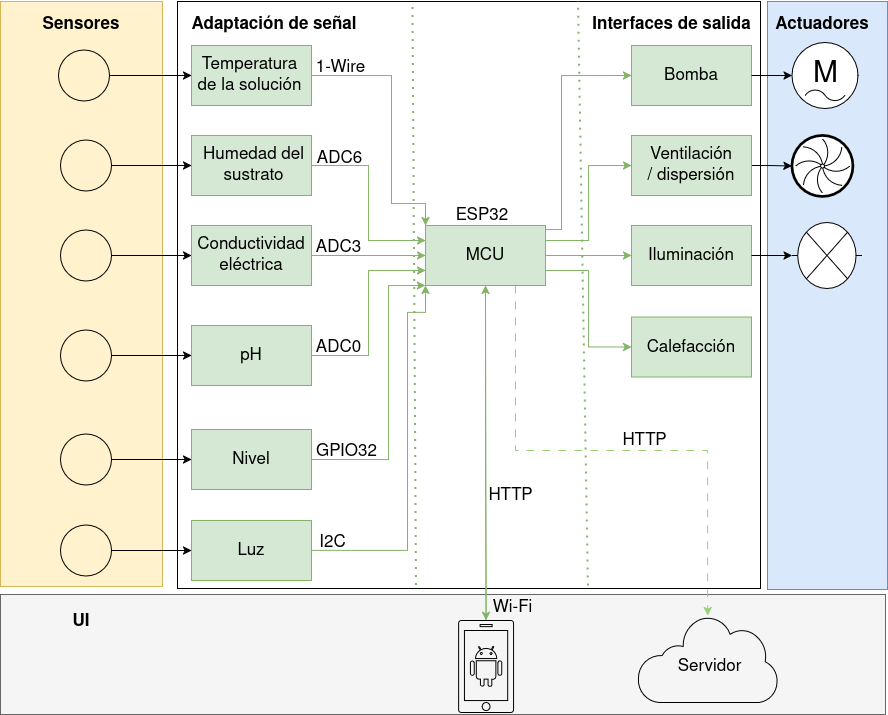
\includegraphics[scale=.5]{./Figures/d_bloques.png}
	\caption{Diagrama de bloques del sistema.}
	\label{fig:d_bloques}
\end{figure}

El sistema embebido implementado en este trabajo consta de una PCB centralizadora, diseñada para integrar y gestionar todos los módulos de hardware. Esta arquitectura asegura la alimentación, adaptación y protección de todos sus componentes. El sistema completo abarca desde la adquisición de datos mediante sensores hasta las acciones sobre el entorno a través de actuadores, y se complementa con una interfaz de usuario móvil para el monitoreo y control remoto.

A continuación, se describen brevemente los bloques y su función.

\begin{itemize}
	\item Sensores: este bloque se encarga de la transducción de magnitudes físicas en señales eléctricas, lo que permite la digitalización de variables ambientales de interés para el control del cultivo.
	\item Adaptación de señal: los módulos de adaptación acondicionan las señales provenientes de los sensores. Para garantizar la correcta interpretación por parte de la unidad de microcontrolador o MCU (del inglés \textit{MicroController Unit}), ajustan los niveles de tensión y la relación señal-ruido a valores apropiados.
	\item MCU: el núcleo del sistema, basado en el chip ESP32, orquesta la comunicación y el control de todos los módulos. Provee la capacidad de procesamiento y la conectividad inalámbrica necesarias para la automatización del cultivo y la interacción con la aplicación móvil.
	\item Interfaces de salida: proporciona aislamiento galvánico y acondicionamiento de potencia para la activación de los actuadores, lo que asegura la protección del MCU y la correcta operación de los componentes de mayor potencia.
	\item Actuadores: los actuadores (ventiladores, bomba de irrigación, luces, resistencia calefactora) ejecutan las acciones de control y modifican las condiciones ambientales del cultivo según las necesidades.
	\item Aplicación móvil de usuario: desarrollada para facilitar la interacción con el sistema, la aplicación móvil permite el monitoreo en tiempo real de las condiciones del cultivo y el control remoto de los actuadores.
	\item Interfaz de servicio web: se implementó una interfaz para la transmisión de datos a un servicio web externo que permite el almacenamiento y análisis de información del cultivo. Esta funcionalidad se encuentra fuera del alcance principal de este trabajo.

\end{itemize}

\section{Arquitectura del firmware}

En la presente sección se aborda la arquitectura del firmware del microcontrolador.

\subsection{Patrones}

Patrones de diseño arquitectónico utilizados.

\subsubsection{Arquitectura en capas}
Se adoptó un patrón de arquitectura en capas para estructurar el software desarrollado, esto permitió una separación de funcionalidades clara mediante niveles de abstracción. Dicha metodología divide el sistema en niveles horizontales, cada uno con responsabilidades específicas y bien definidas, lo que facilita el desarrollo, la mantenibilidad y la escalabilidad del código.

A continuación, las capas de abstracción que constituyen el firmware.

\begin{itemize}
	\item Capa de aplicación.
	\item Capa de sistema operativo.
	\item Capa de abstracción de hardware (HAL).
\end{itemize}


\subsubsection{Capa de abstracción de hardware}

Para facilitar la interacción con los diversos componentes de hardware y garantizar la portabilidad del código, se implementó una capa de abstracción basada en Espressif HAL (\textit{Hardware Abstraction Layer}). Integrada dentro del SDK de ESP-IDF, esta capa proporciona una interfaz uniforme para el control de los periféricos del ESP32, independientemente de las particularidades del hardware subyacente.

\subsubsection{Control ambiental}

El patrón de control ambiental se adoptó como estrategia arquitectónica para la capa de aplicación. El sistema embebido requirió la monitorización y modificación del entorno mediante sensores y actuadores. Este patrón permitió la estructuración de la lógica de control y facilitó la gestión de las interacciones entre los componentes de hardware y la implementación de los algoritmos de control.

\begin{figure}[h]
\centering
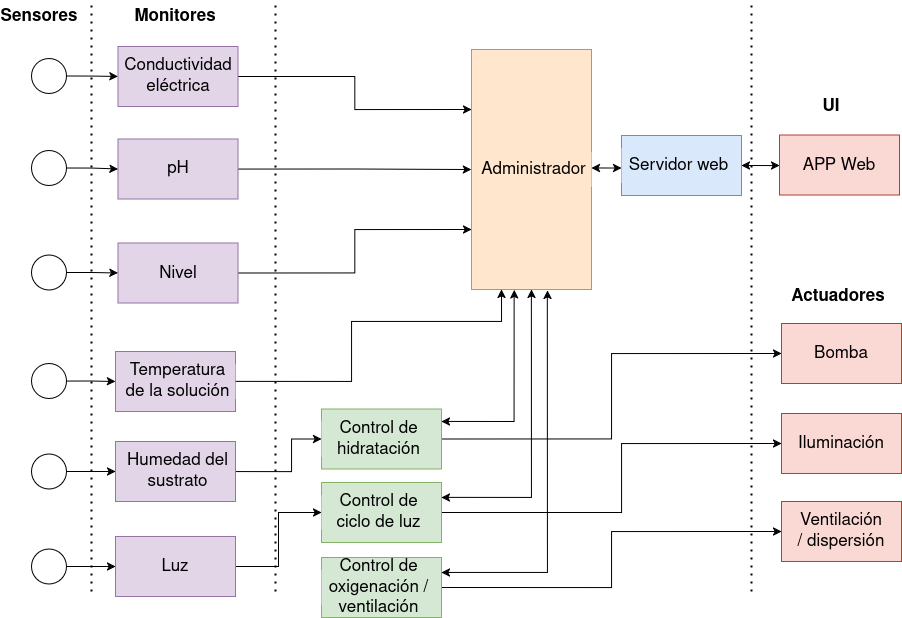
\includegraphics[scale=.5]{./Figures/arq_bloques.png}
	\caption{Diagrama de módulos funcionales y sus interacciones.}
	\label{fig:d_bloques}
\end{figure}

Si en el texto se hace alusión a diferentes partes del trabajo referirse a ellas como capítulo, sección o subsección según corresponda. Por ejemplo: ``En el capítulo \ref{Chapter1} se explica tal cosa'', o ``En la sección \ref{sec:ejemplo} se presenta lo que sea'', o ``En la subsección \ref{subsec:ejemplo} se discute otra cosa''.

Cuando se quiere poner una lista tabulada, se hace así:

\begin{itemize}
	\item Este es el primer elemento de la lista.
	\item Este es el segundo elemento de la lista.
\end{itemize}

Notar el uso de las mayúsculas y el punto al final de cada elemento.

Si se desea poner una lista numerada el formato es este:

\begin{enumerate}
	\item Este es el primer elemento de la lista.
	\item Este es el segundo elemento de la lista.
\end{enumerate}

Notar el uso de las mayúsculas y el punto al final de cada elemento.

\subsection{Este es el título de una subsección}
\label{subsec:ejemplo}

Se recomienda no utilizar \textbf{texto en negritas} en ningún párrafo, ni tampoco texto \underline{subrayado}. En cambio sí se debe utilizar \textit{texto en itálicas} para palabras en un idioma extranjero, al menos la primera vez que aparecen en el texto. En el caso de palabras que estamos inventando se deben utilizar ``comillas'', así como también para citas textuales. Por ejemplo, un \textit{digital filter} es una especie de ``selector'' que permite separar ciertos componentes armónicos en particular.

La escritura debe ser impersonal. Por ejemplo, no utilizar ``el diseño del firmware lo hice de acuerdo con tal principio'', sino ``el firmware fue diseñado utilizando tal principio''. 

El trabajo es algo que al momento de escribir la memoria se supone que ya está concluido, entonces todo lo que se refiera a hacer el trabajo se narra en tiempo pasado, porque es algo que ya ocurrió. Por ejemplo, "se diseñó el firmware empleando la técnica de test driven development".

En cambio, la memoria es algo que está vivo cada vez que el lector la lee. Por eso transcurre siempre en tiempo presente, como por ejemplo:

``En el presente capítulo se da una visión global sobre las distintas pruebas realizadas y los resultados obtenidos. Se explica el modo en que fueron llevados a cabo los test unitarios y las pruebas del sistema''.

Se recomienda no utilizar una sección de glosario sino colocar la descripción de las abreviaturas como parte del mismo cuerpo del texto. Por ejemplo, RTOS (\textit{Real Time Operating System}, Sistema Operativo de Tiempo Real) o en caso de considerarlo apropiado mediante notas a pie de página.

Si se desea indicar alguna página web utilizar el siguiente formato de referencias bibliográficas, dónde las referencias se detallan en la sección de bibliografía de la memoria, utilizado el formato establecido por IEEE en \citep{IEEE:citation}. Por ejemplo, ``el presente trabajo se basa en la plataforma EDU-CIAA-NXP \citep{CIAA}, la cual...''.

\subsection{Figuras} 

Al insertar figuras en la memoria se deben considerar determinadas pautas. Para empezar, usar siempre tipografía claramente legible. Luego, tener claro que \textbf{es incorrecto} escribir por ejemplo esto: ``El diseño elegido es un cuadrado, como se ve en la siguiente figura:''

\begin{figure}[h]
\centering
\includegraphics[scale=.45]{./Figures/cuadradoAzul.png}
\end{figure}

La forma correcta de utilizar una figura es con referencias cruzadas, por ejemplo: ``Se eligió utilizar un cuadrado azul para el logo, como puede observarse en la figura \ref{fig:cuadradoAzul}''.

\begin{figure}[ht]
	\centering
	\includegraphics[scale=.45]{./Figures/cuadradoAzul.png}
	\caption{Ilustración del cuadrado azul que se eligió para el diseño del logo.}
	\label{fig:cuadradoAzul}
\end{figure}

El texto de las figuras debe estar siempre en español, excepto que se decida reproducir una figura original tomada de alguna referencia. En ese caso la referencia de la cual se tomó la figura debe ser indicada en el epígrafe de la figura e incluida como una nota al pie, como se ilustra en la figura \ref{fig:palabraIngles}.

\begin{figure}[htpb]
	\centering
	\includegraphics[scale=.3]{./Figures/word.jpeg}
	\caption{Imagen tomada de la página oficial del procesador\protect\footnotemark.}
	\label{fig:palabraIngles}
\end{figure}

\footnotetext{Imagen tomada de \url{https://goo.gl/images/i7C70w}}

La figura y el epígrafe deben conformar una unidad cuyo significado principal pueda ser comprendido por el lector sin necesidad de leer el cuerpo central de la memoria. Para eso es necesario que el epígrafe sea todo lo detallado que corresponda y si en la figura se utilizan abreviaturas entonces aclarar su significado en el epígrafe o en la misma figura.



\begin{figure}[ht]
	\centering
	\includegraphics[scale=.37]{./Figures/questionMark.png}
	\caption{¿Por qué de pronto aparece esta figura?}
	\label{fig:questionMark}
\end{figure}

Nunca colocar una figura en el documento antes de hacer la primera referencia a ella, como se ilustra con la figura \ref{fig:questionMark}, porque sino el lector no comprenderá por qué de pronto aparece la figura en el documento, lo que distraerá su atención.

Otra posibilidad es utilizar el entorno \textit{subfigure} para incluir más de una figura, como se puede ver en la figura \ref{fig:three graphs}. Notar que se pueden referenciar también las figuras internas individualmente de esta manera: \ref{fig:1de3}, \ref{fig:2de3} y \ref{fig:3de3}.
 
\begin{figure}[!htpb]
     \centering
     \begin{subfigure}[b]{0.3\textwidth}
         \centering
         \includegraphics[width=.65\textwidth]{./Figures/questionMark}
         \caption{Un caption.}
         \label{fig:1de3}
     \end{subfigure}
     \hfill
     \begin{subfigure}[b]{0.3\textwidth}
         \centering
         \includegraphics[width=.65\textwidth]{./Figures/questionMark}
         \caption{Otro.}
         \label{fig:2de3}
     \end{subfigure}
     \hfill
     \begin{subfigure}[b]{0.3\textwidth}
         \centering
         \includegraphics[width=.65\textwidth]{./Figures/questionMark}
         \caption{Y otro más.}
         \label{fig:3de3}
     \end{subfigure}
        \caption{Tres gráficos simples.}
        \label{fig:three graphs}
\end{figure}

El código para generar las imágenes se encuentra disponible para su reutilización en el archivo \file{Chapter2.tex}.

\subsection{Tablas}

Para las tablas utilizar el mismo formato que para las figuras, sólo que el epígrafe se debe colocar arriba de la tabla, como se ilustra en la tabla \ref{tab:peces}. Observar que sólo algunas filas van con líneas visibles y notar el uso de las negritas para los encabezados.  La referencia se logra utilizando el comando \verb|\ref{<label>}| donde label debe estar definida dentro del entorno de la tabla.

\begin{verbatim}
\begin{table}[h]
	\centering
	\caption[caption corto]{caption largo más descriptivo}
	\begin{tabular}{l c c}    
		\toprule
		\textbf{Especie}     & \textbf{Tamaño} & \textbf{Valor}\\
		\midrule
		Amphiprion Ocellaris & 10 cm           & \$ 6.000 \\		
		Hepatus Blue Tang    & 15 cm           & \$ 7.000 \\
		Zebrasoma Xanthurus  & 12 cm           & \$ 6.800 \\
		\bottomrule
		\hline
	\end{tabular}
	\label{tab:peces}
\end{table}
\end{verbatim}


\begin{table}[h]
	\centering
	\caption[caption corto]{caption largo más descriptivo.}
	\begin{tabular}{l c c}    
		\toprule
		\textbf{Especie} 	 & \textbf{Tamaño} 		& \textbf{Valor}  \\
		\midrule
		Amphiprion Ocellaris & 10 cm 				& \$ 6.000 \\		
		Hepatus Blue Tang	 & 15 cm				& \$ 7.000 \\
		Zebrasoma Xanthurus	 & 12 cm				& \$ 6.800 \\
		\bottomrule
		\hline
	\end{tabular}
	\label{tab:peces}
\end{table}

En cada capítulo se debe reiniciar el número de conteo de las figuras y las tablas, por ejemplo, figura 2.1 o tabla 2.1, pero no se debe reiniciar el conteo en cada sección. Por suerte la plantilla se encarga de esto por nosotros.

\subsection{Ecuaciones}
\label{sec:Ecuaciones}

Al insertar ecuaciones en la memoria dentro de un entorno \textit{equation}, éstas se numeran en forma automática  y se pueden referir al igual que como se hace con las figuras y tablas, por ejemplo ver la ecuación \ref{eq:metric}.

\begin{equation}
	\label{eq:metric}
	ds^2 = c^2 dt^2 \left( \frac{d\sigma^2}{1-k\sigma^2} + \sigma^2\left[ d\theta^2 + \sin^2\theta d\phi^2 \right] \right)
\end{equation}
                                                        
Es importante tener presente que si bien las ecuaciones pueden ser referidas por su número, también es correcto utilizar los dos puntos, como por ejemplo ``la expresión matemática que describe este comportamiento es la siguiente:''

\begin{equation}
	\label{eq:schrodinger}
	\frac{\hbar^2}{2m}\nabla^2\Psi + V(\mathbf{r})\Psi = -i\hbar \frac{\partial\Psi}{\partial t}
\end{equation}

Para generar la ecuación \ref{eq:metric} se utilizó el siguiente código:

\begin{verbatim}
\begin{equation}
	\label{eq:metric}
	ds^2 = c^2 dt^2 \left( \frac{d\sigma^2}{1-k\sigma^2} + 
	\sigma^2\left[ d\theta^2 + 
	\sin^2\theta d\phi^2 \right] \right)
\end{equation}
\end{verbatim}

Y para la ecuación \ref{eq:schrodinger}:

\begin{verbatim}
\begin{equation}
	\label{eq:schrodinger}
	\frac{\hbar^2}{2m}\nabla^2\Psi + V(\mathbf{r})\Psi = 
	-i\hbar \frac{\partial\Psi}{\partial t}
\end{equation}

\end{verbatim}

\definecolor{mygreen}{rgb}{0,0.6,0}
\definecolor{mygray}{rgb}{0.5,0.5,0.5}
\definecolor{mymauve}{rgb}{0.58,0,0.82}

%%%%%%%%%%%%%%%%%%%%%%%%%%%%%%%%%%%%%%%%%%%%%%%%%%%%%%%%%%%%%%%%%%%%%%%%%%%%%
% parámetros para configurar el formato del código en los entornos lstlisting
%%%%%%%%%%%%%%%%%%%%%%%%%%%%%%%%%%%%%%%%%%%%%%%%%%%%%%%%%%%%%%%%%%%%%%%%%%%%%
\lstset{ %
  backgroundcolor=\color{white},   % choose the background color; you must add \usepackage{color} or \usepackage{xcolor}
  basicstyle=\footnotesize,        % the size of the fonts that are used for the code
  breakatwhitespace=false,         % sets if automatic breaks should only happen at whitespace
  breaklines=true,                 % sets automatic line breaking
  captionpos=b,                    % sets the caption-position to bottom
  commentstyle=\color{mygreen},    % comment style
  deletekeywords={...},            % if you want to delete keywords from the given language
  %escapeinside={\%*}{*)},          % if you want to add LaTeX within your code
  %extendedchars=true,              % lets you use non-ASCII characters; for 8-bits encodings only, does not work with UTF-8
  %frame=single,	                % adds a frame around the code
  keepspaces=true,                 % keeps spaces in text, useful for keeping indentation of code (possibly needs columns=flexible)
  keywordstyle=\color{blue},       % keyword style
  language=[ANSI]C,                % the language of the code
  %otherkeywords={*,...},           % if you want to add more keywords to the set
  numbers=left,                    % where to put the line-numbers; possible values are (none, left, right)
  numbersep=5pt,                   % how far the line-numbers are from the code
  numberstyle=\tiny\color{mygray}, % the style that is used for the line-numbers
  rulecolor=\color{black},         % if not set, the frame-color may be changed on line-breaks within not-black text (e.g. comments (green here))
  showspaces=false,                % show spaces everywhere adding particular underscores; it overrides 'showstringspaces'
  showstringspaces=false,          % underline spaces within strings only
  showtabs=false,                  % show tabs within strings adding particular underscores
  stepnumber=1,                    % the step between two line-numbers. If it's 1, each line will be numbered
  stringstyle=\color{mymauve},     % string literal style
  tabsize=2,	                   % sets default tabsize to 2 spaces
  title=\lstname,                  % show the filename of files included with \lstinputlisting; also try caption instead of title
  morecomment=[s]{/*}{*/}
}


%----------------------------------------------------------------------------------------
%	SECTION 1
%----------------------------------------------------------------------------------------
\section{Análisis del software}
 
La idea de esta sección es resaltar los problemas encontrados, los criterios utilizados y la justificación de las decisiones que se hayan tomado.

Se puede agregar código o pseudocódigo dentro de un entorno lstlisting con el siguiente código:

\begin{verbatim}
\begin{lstlisting}[caption= "un epígrafe descriptivo"]
	las líneas de código irían aquí...
\end{lstlisting}
\end{verbatim}

A modo de ejemplo:

\begin{lstlisting}[label=cod:vControl,caption=Pseudocódigo del lazo principal de control.]  % Start your code-block

#define MAX_SENSOR_NUMBER 3
#define MAX_ALARM_NUMBER  6
#define MAX_ACTUATOR_NUMBER 6

uint32_t sensorValue[MAX_SENSOR_NUMBER];		
FunctionalState alarmControl[MAX_ALARM_NUMBER];	//ENABLE or DISABLE
state_t alarmState[MAX_ALARM_NUMBER];						//ON or OFF
state_t actuatorState[MAX_ACTUATOR_NUMBER];			//ON or OFF

void vControl() {

	initGlobalVariables();
	
	period = 500 ms;
		
	while(1) {

		ticks = xTaskGetTickCount();
		
		updateSensors();
		
		updateAlarms();
		
		controlActuators();
		
		vTaskDelayUntil(&ticks, period);
	}
}
\end{lstlisting}




% Chapter Template

\chapter{Ensayos y resultados} % Main chapter title

Si en el texto se hace alusión a diferentes partes del trabajo referirse a ellas como capítulo, sección o subsección según corresponda. Por ejemplo: ``En el capítulo \ref{Chapter1} se explica tal cosa'', o ``En la sección \ref{sec:ejemplo} se presenta lo que sea'', o ``En la subsección \ref{subsec:ejemplo} se discute otra cosa''.

Cuando se quiere poner una lista tabulada, se hace así:

\begin{itemize}
	\item Este es el primer elemento de la lista.
	\item Este es el segundo elemento de la lista.
\end{itemize}

Notar el uso de las mayúsculas y el punto al final de cada elemento.

Si se desea poner una lista numerada el formato es este:

\begin{enumerate}
	\item Este es el primer elemento de la lista.
	\item Este es el segundo elemento de la lista.
\end{enumerate}

Notar el uso de las mayúsculas y el punto al final de cada elemento.

\subsection{Este es el título de una subsección}
\label{subsec:ejemplo}

Se recomienda no utilizar \textbf{texto en negritas} en ningún párrafo, ni tampoco texto \underline{subrayado}. En cambio sí se debe utilizar \textit{texto en itálicas} para palabras en un idioma extranjero, al menos la primera vez que aparecen en el texto. En el caso de palabras que estamos inventando se deben utilizar ``comillas'', así como también para citas textuales. Por ejemplo, un \textit{digital filter} es una especie de ``selector'' que permite separar ciertos componentes armónicos en particular.

La escritura debe ser impersonal. Por ejemplo, no utilizar ``el diseño del firmware lo hice de acuerdo con tal principio'', sino ``el firmware fue diseñado utilizando tal principio''. 

El trabajo es algo que al momento de escribir la memoria se supone que ya está concluido, entonces todo lo que se refiera a hacer el trabajo se narra en tiempo pasado, porque es algo que ya ocurrió. Por ejemplo, "se diseñó el firmware empleando la técnica de test driven development".

En cambio, la memoria es algo que está vivo cada vez que el lector la lee. Por eso transcurre siempre en tiempo presente, como por ejemplo:

``En el presente capítulo se da una visión global sobre las distintas pruebas realizadas y los resultados obtenidos. Se explica el modo en que fueron llevados a cabo los test unitarios y las pruebas del sistema''.

Se recomienda no utilizar una sección de glosario sino colocar la descripción de las abreviaturas como parte del mismo cuerpo del texto. Por ejemplo, RTOS (\textit{Real Time Operating System}, Sistema Operativo de Tiempo Real) o en caso de considerarlo apropiado mediante notas a pie de página.

Si se desea indicar alguna página web utilizar el siguiente formato de referencias bibliográficas, dónde las referencias se detallan en la sección de bibliografía de la memoria, utilizado el formato establecido por IEEE en \citep{IEEE:citation}. Por ejemplo, ``el presente trabajo se basa en la plataforma EDU-CIAA-NXP \citep{CIAA}, la cual...''.

\subsection{Figuras} 

Al insertar figuras en la memoria se deben considerar determinadas pautas. Para empezar, usar siempre tipografía claramente legible. Luego, tener claro que \textbf{es incorrecto} escribir por ejemplo esto: ``El diseño elegido es un cuadrado, como se ve en la siguiente figura:''

\begin{figure}[h]
\centering
\includegraphics[scale=.45]{./Figures/cuadradoAzul.png}
\end{figure}

La forma correcta de utilizar una figura es con referencias cruzadas, por ejemplo: ``Se eligió utilizar un cuadrado azul para el logo, como puede observarse en la figura \ref{fig:cuadradoAzul}''.

\begin{figure}[ht]
	\centering
	\includegraphics[scale=.45]{./Figures/cuadradoAzul.png}
	\caption{Ilustración del cuadrado azul que se eligió para el diseño del logo.}
	\label{fig:cuadradoAzul}
\end{figure}

El texto de las figuras debe estar siempre en español, excepto que se decida reproducir una figura original tomada de alguna referencia. En ese caso la referencia de la cual se tomó la figura debe ser indicada en el epígrafe de la figura e incluida como una nota al pie, como se ilustra en la figura \ref{fig:palabraIngles}.

\begin{figure}[htpb]
	\centering
	\includegraphics[scale=.3]{./Figures/word.jpeg}
	\caption{Imagen tomada de la página oficial del procesador\protect\footnotemark.}
	\label{fig:palabraIngles}
\end{figure}

\footnotetext{Imagen tomada de \url{https://goo.gl/images/i7C70w}}

La figura y el epígrafe deben conformar una unidad cuyo significado principal pueda ser comprendido por el lector sin necesidad de leer el cuerpo central de la memoria. Para eso es necesario que el epígrafe sea todo lo detallado que corresponda y si en la figura se utilizan abreviaturas entonces aclarar su significado en el epígrafe o en la misma figura.



\begin{figure}[ht]
	\centering
	\includegraphics[scale=.37]{./Figures/questionMark.png}
	\caption{¿Por qué de pronto aparece esta figura?}
	\label{fig:questionMark}
\end{figure}

Nunca colocar una figura en el documento antes de hacer la primera referencia a ella, como se ilustra con la figura \ref{fig:questionMark}, porque sino el lector no comprenderá por qué de pronto aparece la figura en el documento, lo que distraerá su atención.

Otra posibilidad es utilizar el entorno \textit{subfigure} para incluir más de una figura, como se puede ver en la figura \ref{fig:three graphs}. Notar que se pueden referenciar también las figuras internas individualmente de esta manera: \ref{fig:1de3}, \ref{fig:2de3} y \ref{fig:3de3}.
 
\begin{figure}[!htpb]
     \centering
     \begin{subfigure}[b]{0.3\textwidth}
         \centering
         \includegraphics[width=.65\textwidth]{./Figures/questionMark}
         \caption{Un caption.}
         \label{fig:1de3}
     \end{subfigure}
     \hfill
     \begin{subfigure}[b]{0.3\textwidth}
         \centering
         \includegraphics[width=.65\textwidth]{./Figures/questionMark}
         \caption{Otro.}
         \label{fig:2de3}
     \end{subfigure}
     \hfill
     \begin{subfigure}[b]{0.3\textwidth}
         \centering
         \includegraphics[width=.65\textwidth]{./Figures/questionMark}
         \caption{Y otro más.}
         \label{fig:3de3}
     \end{subfigure}
        \caption{Tres gráficos simples.}
        \label{fig:three graphs}
\end{figure}

El código para generar las imágenes se encuentra disponible para su reutilización en el archivo \file{Chapter2.tex}.

\subsection{Tablas}

Para las tablas utilizar el mismo formato que para las figuras, sólo que el epígrafe se debe colocar arriba de la tabla, como se ilustra en la tabla \ref{tab:peces}. Observar que sólo algunas filas van con líneas visibles y notar el uso de las negritas para los encabezados.  La referencia se logra utilizando el comando \verb|\ref{<label>}| donde label debe estar definida dentro del entorno de la tabla.

\begin{verbatim}
\begin{table}[h]
	\centering
	\caption[caption corto]{caption largo más descriptivo}
	\begin{tabular}{l c c}    
		\toprule
		\textbf{Especie}     & \textbf{Tamaño} & \textbf{Valor}\\
		\midrule
		Amphiprion Ocellaris & 10 cm           & \$ 6.000 \\		
		Hepatus Blue Tang    & 15 cm           & \$ 7.000 \\
		Zebrasoma Xanthurus  & 12 cm           & \$ 6.800 \\
		\bottomrule
		\hline
	\end{tabular}
	\label{tab:peces}
\end{table}
\end{verbatim}


\begin{table}[h]
	\centering
	\caption[caption corto]{caption largo más descriptivo.}
	\begin{tabular}{l c c}    
		\toprule
		\textbf{Especie} 	 & \textbf{Tamaño} 		& \textbf{Valor}  \\
		\midrule
		Amphiprion Ocellaris & 10 cm 				& \$ 6.000 \\		
		Hepatus Blue Tang	 & 15 cm				& \$ 7.000 \\
		Zebrasoma Xanthurus	 & 12 cm				& \$ 6.800 \\
		\bottomrule
		\hline
	\end{tabular}
	\label{tab:peces}
\end{table}

En cada capítulo se debe reiniciar el número de conteo de las figuras y las tablas, por ejemplo, figura 2.1 o tabla 2.1, pero no se debe reiniciar el conteo en cada sección. Por suerte la plantilla se encarga de esto por nosotros.

\subsection{Ecuaciones}
\label{sec:Ecuaciones}

Al insertar ecuaciones en la memoria dentro de un entorno \textit{equation}, éstas se numeran en forma automática  y se pueden referir al igual que como se hace con las figuras y tablas, por ejemplo ver la ecuación \ref{eq:metric}.

\begin{equation}
	\label{eq:metric}
	ds^2 = c^2 dt^2 \left( \frac{d\sigma^2}{1-k\sigma^2} + \sigma^2\left[ d\theta^2 + \sin^2\theta d\phi^2 \right] \right)
\end{equation}
                                                        
Es importante tener presente que si bien las ecuaciones pueden ser referidas por su número, también es correcto utilizar los dos puntos, como por ejemplo ``la expresión matemática que describe este comportamiento es la siguiente:''

\begin{equation}
	\label{eq:schrodinger}
	\frac{\hbar^2}{2m}\nabla^2\Psi + V(\mathbf{r})\Psi = -i\hbar \frac{\partial\Psi}{\partial t}
\end{equation}

Para generar la ecuación \ref{eq:metric} se utilizó el siguiente código:

\begin{verbatim}
\begin{equation}
	\label{eq:metric}
	ds^2 = c^2 dt^2 \left( \frac{d\sigma^2}{1-k\sigma^2} + 
	\sigma^2\left[ d\theta^2 + 
	\sin^2\theta d\phi^2 \right] \right)
\end{equation}
\end{verbatim}

Y para la ecuación \ref{eq:schrodinger}:

\begin{verbatim}
\begin{equation}
	\label{eq:schrodinger}
	\frac{\hbar^2}{2m}\nabla^2\Psi + V(\mathbf{r})\Psi = 
	-i\hbar \frac{\partial\Psi}{\partial t}
\end{equation}

\end{verbatim}

\definecolor{mygreen}{rgb}{0,0.6,0}
\definecolor{mygray}{rgb}{0.5,0.5,0.5}
\definecolor{mymauve}{rgb}{0.58,0,0.82}

%%%%%%%%%%%%%%%%%%%%%%%%%%%%%%%%%%%%%%%%%%%%%%%%%%%%%%%%%%%%%%%%%%%%%%%%%%%%%
% parámetros para configurar el formato del código en los entornos lstlisting
%%%%%%%%%%%%%%%%%%%%%%%%%%%%%%%%%%%%%%%%%%%%%%%%%%%%%%%%%%%%%%%%%%%%%%%%%%%%%
\lstset{ %
  backgroundcolor=\color{white},   % choose the background color; you must add \usepackage{color} or \usepackage{xcolor}
  basicstyle=\footnotesize,        % the size of the fonts that are used for the code
  breakatwhitespace=false,         % sets if automatic breaks should only happen at whitespace
  breaklines=true,                 % sets automatic line breaking
  captionpos=b,                    % sets the caption-position to bottom
  commentstyle=\color{mygreen},    % comment style
  deletekeywords={...},            % if you want to delete keywords from the given language
  %escapeinside={\%*}{*)},          % if you want to add LaTeX within your code
  %extendedchars=true,              % lets you use non-ASCII characters; for 8-bits encodings only, does not work with UTF-8
  %frame=single,	                % adds a frame around the code
  keepspaces=true,                 % keeps spaces in text, useful for keeping indentation of code (possibly needs columns=flexible)
  keywordstyle=\color{blue},       % keyword style
  language=[ANSI]C,                % the language of the code
  %otherkeywords={*,...},           % if you want to add more keywords to the set
  numbers=left,                    % where to put the line-numbers; possible values are (none, left, right)
  numbersep=5pt,                   % how far the line-numbers are from the code
  numberstyle=\tiny\color{mygray}, % the style that is used for the line-numbers
  rulecolor=\color{black},         % if not set, the frame-color may be changed on line-breaks within not-black text (e.g. comments (green here))
  showspaces=false,                % show spaces everywhere adding particular underscores; it overrides 'showstringspaces'
  showstringspaces=false,          % underline spaces within strings only
  showtabs=false,                  % show tabs within strings adding particular underscores
  stepnumber=1,                    % the step between two line-numbers. If it's 1, each line will be numbered
  stringstyle=\color{mymauve},     % string literal style
  tabsize=2,	                   % sets default tabsize to 2 spaces
  title=\lstname,                  % show the filename of files included with \lstinputlisting; also try caption instead of title
  morecomment=[s]{/*}{*/}
}


%----------------------------------------------------------------------------------------
%	SECTION 1
%----------------------------------------------------------------------------------------
\section{Análisis del software}
 
La idea de esta sección es resaltar los problemas encontrados, los criterios utilizados y la justificación de las decisiones que se hayan tomado.

Se puede agregar código o pseudocódigo dentro de un entorno lstlisting con el siguiente código:

\begin{verbatim}
\begin{lstlisting}[caption= "un epígrafe descriptivo"]
	las líneas de código irían aquí...
\end{lstlisting}
\end{verbatim}

A modo de ejemplo:

\begin{lstlisting}[label=cod:vControl,caption=Pseudocódigo del lazo principal de control.]  % Start your code-block

#define MAX_SENSOR_NUMBER 3
#define MAX_ALARM_NUMBER  6
#define MAX_ACTUATOR_NUMBER 6

uint32_t sensorValue[MAX_SENSOR_NUMBER];		
FunctionalState alarmControl[MAX_ALARM_NUMBER];	//ENABLE or DISABLE
state_t alarmState[MAX_ALARM_NUMBER];						//ON or OFF
state_t actuatorState[MAX_ACTUATOR_NUMBER];			//ON or OFF

void vControl() {

	initGlobalVariables();
	
	period = 500 ms;
		
	while(1) {

		ticks = xTaskGetTickCount();
		
		updateSensors();
		
		updateAlarms();
		
		controlActuators();
		
		vTaskDelayUntil(&ticks, period);
	}
}
\end{lstlisting}





\label{Chapter4} % Change X to a consecutive number; for referencing this chapter elsewhere, use \ref{ChapterX}
Todos los capítulos deben comenzar con un breve párrafo introductorio que indique cuál es el contenido que se encontrará al leerlo.  La redacción sobre el contenido de la memoria debe hacerse en presente y todo lo referido al proyecto en pasado, siempre de modo impersonal.

%----------------------------------------------------------------------------------------
%	SECTION 1
%----------------------------------------------------------------------------------------

\section{Pruebas funcionales del hardware}
\label{sec:pruebasHW}

La idea de esta sección es explicar cómo se hicieron los ensayos, qué resultados se obtuvieron y analizarlos.

% Chapter Template

\chapter{Conclusiones} % Main chapter title

\label{Chapter5} % Change X to a consecutive number; for referencing this chapter elsewhere, use \ref{ChapterX}
Todos los capítulos deben comenzar con un breve párrafo introductorio que indique cuál es el contenido que se encontrará al leerlo.  La redacción sobre el contenido de la memoria debe hacerse en presente y todo lo referido al proyecto en pasado, siempre de modo impersonal.


%----------------------------------------------------------------------------------------

%----------------------------------------------------------------------------------------
%	SECTION 1
%----------------------------------------------------------------------------------------

\section{Conclusiones generales }

La idea de esta sección es resaltar cuáles son los principales aportes del trabajo realizado y cómo se podría continuar. Debe ser especialmente breve y concisa. Es buena idea usar un listado para enumerar los logros obtenidos.

En esta sección no se deben incluir ni tablas ni gráficos.

Algunas preguntas que pueden servir para completar este capítulo:

\begin{itemize}
\item ¿Cuál es el grado de cumplimiento de los requerimientos?
\item ¿Cuán fielmente se puedo seguir la planificación original (cronograma incluido)?
\item ¿Se manifestó algunos de los riesgos identificados en la planificación? ¿Fue efectivo el plan de mitigación? ¿Se debió aplicar alguna otra acción no contemplada previamente?
\item Si se debieron hacer modificaciones a lo planificado ¿Cuáles fueron las causas y los efectos?
\item ¿Qué técnicas resultaron útiles para el desarrollo del proyecto y cuáles no tanto?
\end{itemize}


%----------------------------------------------------------------------------------------
%	SECTION 2
%----------------------------------------------------------------------------------------
\section{Próximos pasos}

Acá se indica cómo se podría continuar el trabajo más adelante.

Este es un ejemplo de cita de un artículo \cite{ARTICLE:1}.  
Aquí citamos un libro \cite{BOOK:1} y un capítulo de libro \cite{BOOK:2}.  
También podemos citar una página web \cite{WEBSITE:1}.  
O una referencia de un manual técnico \cite{dallas:ds18b20}.

%----------------------------------------------------------------------------------------
% Apéndices
%----------------------------------------------------------------------------------------

\appendix

% Incluir apéndices desde archivos separados si es necesario
%\include{Appendices/AppendixA}

%----------------------------------------------------------------------------------------
% Bibliografía
%----------------------------------------------------------------------------------------

\renewcommand{\bibname}{Bibliografía} % Para asegurarte de que el título sea correcto
\phantomsection % Necesario para que el enlace del marcador sea correcto

\printbibliography[heading=bibintoc]

\end{document}






